\documentclass{article}
\usepackage[utf8]{inputenc}
\usepackage{subcaption}
\usepackage{listings}
\usepackage{geometry}
\usepackage[bottom]{footmisc}
\usepackage{verbatim}
\usepackage{amsmath}
\usepackage{amssymb}
\usepackage{amsfonts}
% allows table of contents to be clickable
\usepackage{hyperref}
\hypersetup{
    colorlinks=true,
    linkcolor=blue,
    filecolor=magenta,      
    urlcolor=blue,
    citecolor=blue,
}
\usepackage{mdframed}
% allows for figures and captions
\usepackage{graphicx}
\usepackage{caption}
\usepackage{dblfloatfix}
% allows to specify which token to use in enumerate
\usepackage{enumitem}
\DeclareMathOperator*{\argmax}{arg\,max}
\DeclareMathOperator*{\argmin}{arg\,min}
\usepackage{pythonhighlight} % python code highlighting using \begin{python}
\usepackage{accents}

% for automatically making an index for notes (use \printindex at end of document
\usepackage{makeidx}
\makeindex

% independence symbol
% usage:
% X \independent{Y}
\newcommand\independent{\protect\mathpalette{\protect\independenT}{\perp}}
\def\independenT#1#2{\mathrel{\rlap{$#1#2$}\mkern2mu{#1#2}}}

% augmented matrices
% usage:
% \begin{amatrix}{#columns - 1} \end{amatrix}
\newenvironment{amatrix}[1]{%
  \left(\begin{array}{@{}*{#1}{c}|c@{}}
}{%
  \end{array}\right)
}

% Theorem and Definition Frames
% usage:
% \begin{theo} \end{theo}
% \begin{define} \end{define}
\newmdtheoremenv{theo}{Theorem}
\newmdtheoremenv{thm}{Theorem}
\newmdtheoremenv{define}{Definition}
\newmdtheoremenv{alg}{Algorithm}
\newmdtheoremenv{lem}{Lemma}
\newmdtheoremenv{proof}{Proof}
\newmdtheoremenv{cor}{Corollary}
\newmdtheoremenv{claim}{Claim}
\newmdtheoremenv{rem}{Remark}



% Figure Drawing Packages
\usepackage{tikz}
\usepackage{pgfplots}
\pgfplotsset{width=10cm,compat=1.9}


% Proof environment with [] ending
\newenvironment{Proof}{\noindent {\sc Proof:}}{$\Box$ \vspace{2 ex}}

% Draw a horizontal bar across length of page
\newcommand{\hacross}{\noindent\rule{15.2cm}{0.4pt}\\}

% Useful packages for drawing commutative diagrams!
%\usepackage{pst-node}
%\usepackage{auto-pst-pdf}
%\usepackage{tikz-cd} 

% Change text colors conveniently
\newcommand{\red}[1]{\textcolor{red}{#1}}
\newcommand{\blue}[1]{\textcolor{blue}{#1}}


% Shortcuts for commonly used phrases

\newcommand{\spfc}{Suppose for the purpose of contradiction }
\newcommand{\tfae}{Then the following are equivalent:}


%%%%% Notation page
\usepackage{nomencl}
\makenomenclature




%%%%%%%%%  STAT 210B Style commands
%%% Math commands

% Probability
\renewcommand{\P}{\mathbb{P}}
% Expectation
\newcommand{\E}{\mathbb{E}}
% Variance
\newcommand{\Var}{\text{Var}}
% Covariance. 
\newcommand{\Cov}{\text{Cov}}
% Normal distribution. Example: $X_i \sim_{iid} \cN(0, 1)$. 
\newcommand{\cN}{\mathcal{N}}

%% Sets
% Integers
\newcommand{\Z}{\mathbb{Z}}
% Reals
\newcommand{\R}{\mathbb{R}}
% Complex
\newcommand{\C}{\mathbb{C}}
% Natural
\newcommand{\N}{\mathbb{N}}
% Sphere. Example: $\S^{d-1}(\sqrt{d})$. 
\renewcommand{\S}{\mathbb{S}}
% Ball. Example: $\ball(0, 1)$. 
\def\ball{{\mathsf B}}


%% Math
% Inner products
\newcommand{\<}{\langle}
\renewcommand{\>}{\rangle}
% Trace. Example: $\tr(\bA)$
\newcommand{\tr}{\text{tr}}
% Operator norm. Example: $\| \bA \|_{\op}$. 
\newcommand{\op}{{\rm op}}
% Indicator function. Example: $\ones\{ A > 1 \}$. 
\newcommand{\ones}{\bm{1}}
% Wide hat.
\newcommand{\what}{\widehat}
% Matrix transpose. Example: $\bA^\sT$. 
\def\sT{{\mathsf T}}
% Zero matrix. 
\def\bzero{{\boldsymbol 0}}
% Identically distributed as. Example: $X_i \simiid \cN(0, 1)$. 
\def\simiid{\sim_{i.i.d.}}
% sign
\def\sign{{\rm sign}}
% integral d: Example: $\int_\R f(x) \de x$. 
\def\de{{\rm d}}
% Uniform distribution. 
\def\Unif{{\rm Unif}}


% Variables
\def\ba{{\boldsymbol a}}
\def\boldb{{\boldsymbol b}}
\def\bc{{\boldsymbol c}}
\def\bd{{\boldsymbol d}}
\def\be{{\boldsymbol e}}
\def\boldf{{\boldsymbol f}}
\def\bg{{\boldsymbol g}}
\def\bh{{\boldsymbol h}}
\def\bi{{\boldsymbol i}}
\def\bj{{\boldsymbol j}}
\def\bk{{\boldsymbol k}}
\def\bl{{\boldsymbol l}}
\def\boldm{{\boldsymbol m}}
\def\bn{{\boldsymbol n}}
\def\bo{{\boldsymbol o}}
\def\bp{{\boldsymbol p}}
\def\bq{{\boldsymbol q}}
\def\br{{\boldsymbol r}}
\def\bs{{\boldsymbol s}}
\def\bt{{\boldsymbol t}}
\def\bu{{\boldsymbol u}}
\def\bv{{\boldsymbol v}}
\def\bw{{\boldsymbol w}}
\def\bx{{\boldsymbol x}}
\def\by{{\boldsymbol y}}
\def\bz{{\boldsymbol z}}
\def\bA{{\boldsymbol A}}
\def\bB{{\boldsymbol B}}
\def\bC{{\boldsymbol C}}
\def\bD{{\boldsymbol D}}
\def\bE{{\boldsymbol E}}
\def\bF{{\boldsymbol F}}
\def\bG{{\boldsymbol G}}
\def\bH{{\boldsymbol H}}
\def\bI{{\boldsymbol I}}
\def\bJ{{\boldsymbol J}}
\def\bK{{\boldsymbol K}}
\def\bL{{\boldsymbol L}}
\def\bM{{\boldsymbol M}}
\def\bN{{\boldsymbol N}}
\def\bO{{\boldsymbol O}}
\def\bP{{\boldsymbol P}}
\def\bQ{{\boldsymbol Q}}
\def\bR{{\boldsymbol R}}
\def\bS{{\boldsymbol S}}
\def\bT{{\boldsymbol T}}
\def\bU{{\boldsymbol U}}
\def\bV{{\boldsymbol V}}
\def\bW{{\boldsymbol W}}
\def\bX{{\boldsymbol X}}
\def\bY{{\boldsymbol Y}}
\def\bZ{{\boldsymbol Z}}

\def\bsigma{{\boldsymbol \sigma}}
\def\bphi{{\boldsymbol \phi}}
\def\bpsi{{\boldsymbol \psi}}
\def\blambda{{\boldsymbol \lambda}}
\def\beps{{\boldsymbol \eps}}
\def\bmu{{\boldsymbol \mu}}
\def\bxi{{\boldsymbol \xi}}
\def\btheta{{\boldsymbol \theta}}
\def\bbeta{{\boldsymbol \beta}}
\def\boldeta{{\boldsymbol \eta}}
\def\bnu{{\boldsymbol \nu}}
\def\bdelta{{\boldsymbol \deta}}

\def\bTheta{{\boldsymbol \Theta}}
\def\bSigma{{\boldsymbol \Sigma}}
\def\bDelta{{\boldsymbol \Delta}}
\def\bLambda{{\boldsymbol \Lambda}}
\def\bPhi{{\boldsymbol \Phi}}
\def\bPsi{{\boldsymbol \Psi}}
\def\bXi{{\boldsymbol \Xi}}

\def\cA{{\mathcal A}}
\def\cB{{\mathcal B}}
\def\cC{{\mathcal C}}
\def\cD{{\mathcal D}}
\def\cE{{\mathcal E}}
\def\cF{{\mathcal F}}
\def\cG{{\mathcal G}}
\def\cH{{\mathcal H}}
\def\cI{{\mathcal I}}
\def\cJ{{\mathcal J}}
\def\cK{{\mathcal K}}
\def\cL{{\mathcal L}}
\def\cM{{\mathcal M}}
\def\cN{{\mathcal N}}
\def\cO{{\mathcal O}}
\def\cP{{\mathcal P}}
\def\cQ{{\mathcal Q}}
\def\cR{{\mathcal R}}
\def\cS{{\mathcal S}}
\def\cT{{\mathcal T}}
\def\cU{{\mathcal U}}
\def\cV{{\mathcal V}}
\def\cW{{\mathcal W}}
\def\cX{{\mathcal X}}
\def\cY{{\mathcal Y}}
\def\cZ{{\mathcal Z}}

\newcommand{\eps}{\varepsilon} 
\newcommand{\vphi}{\varphi}
\def\id{{\mathbf I}}



\DeclareMathOperator*{\argsup}{arg\,sup}
\DeclareMathOperator*{\arginf}{arg\,inf}


\usepackage[authoryear,square]{natbib}
\usetikzlibrary{positioning}


\title{Brownian Motion, Bridges, and Bayesian Inference in Phylogenetic Tree Space}
\author{Zachary McNulty}
\date{November 2025}


%%%%%%% presentation specific commands

\begin{document}

\maketitle

\hacross

\noindent These notes are based on the paper
\cite{woodman2025brownianmotionbridgesbayesian}, together with some additional
background and motivation.

\section{Background}

The goal of phylogenetics is to use information about a collection of species
to infer their evolutionary history: the shared ancestors and speciation events
that produced the species observed today. We are typically interested in both
the \textit{topology} of the evolutionary tree, which records the sequence of
speciation events, and its \textit{metric structure}, which records the elapsed
time between them. Historically, inference relied on morphological features,
from skeletal structures to plumage patterns. Today, genetic sequence data play
an increasingly predominant role.

Given aligned DNA sequences for a particular gene across several species, one
can specify a model of sequence evolution and select the tree with the largest
likelihood. For example, the Jukes--Cantor model assumes that each nucleotide in
$\{A,C,G,T\}$ changes to any of the other three at the same rate. With genome-scale
data, however, different genes can support substantially different tree
topologies. We therefore need procedures that aggregate information across gene
trees.

The simplest approach is concatenation, which treats all available sequence
data as one long alignment and applies maximum likelihood once. Consensus
methods instead estimate a tree for each gene and use the resulting collection
as input to a second procedure. For example, ASTRAL
\cite{mirarab2014astral} seeks a species tree that maximizes its quartet
agreement with the gene trees:
%
\[\widehat{T}=\arg\max_T\sum_{g\in\cG}
  \operatorname{qscore}(g,T).\]
%
\noindent Although many consensus methods are asymptotically consistent,
finite-sample guarantees can be difficult to obtain, and their statistical
analysis is often tailored to the particular combinatorial procedure.

Ideally, we would like to adapt familiar tools such as concentration of sample
means, principal component analysis, and Bayesian inference. Doing so directly
in a discrete space with little geometry is difficult. To see what goes wrong,
we begin with Fr\'echet means and then introduce the geometric model used in the
paper.

\begin{figure}[b]
    \centering
    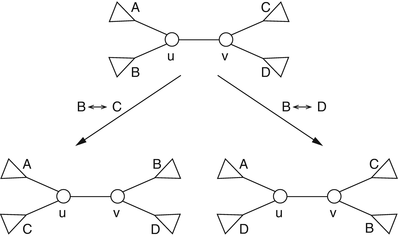
\includegraphics[width=0.5\linewidth]{images/NNI.png}
    \caption{An example of two possible NNI moves.}
    \label{fig:nni_move}
\end{figure}


% Frechet Means
\subsection{Fr\'echet Means}

\noindent Recall that in $\mathbb{R}^d$ the sample mean $\overline{x}$ of data points $\{x_i\}_{i=1}^n$ has the variational characterization:
%
\[\overline{x} = \arg\min_{c \in \R^d} \sum_{i=1}^n ||x_i - c||_2^2\]
%
\noindent This is just a consequence of the bias-variance decomposition of squared error. Likewise, we can extend this to the population level. Given a probability distribution $\mu$ on $\R^d$ we know: 
%
\[ \E_{X \sim \mu} X = \arg \min_{c \in \mathbb{R}^d} \E_{X \sim \mu} ||X - c||_2^2\]
%
\noindent The sample identity is the special case in which $\mu$ is the
empirical distribution of $\{x_i\}$. The \textit{Fr\'echet mean} extends the
ordinary Euclidean mean to a metric space $(\cX,d)$. We define an empirical
Fr\'echet mean by
%
\[\overline{x} := \arg \min_{c \in \cX} \sum_{i=1}^n d(x_i, c)^2\]
%
\noindent and define the population version analogously. Under suitable
geometric and moment assumptions, the Fr\'echet mean exists, is unique, and
enjoys concentration properties analogous to those of the Euclidean sample
mean.

\begin{thm}[Fr\'echet means]
    Let $(\cX,d)$ be a complete $CAT(0)$ space, and suppose that $\mu$ has
    finite second moment. Then the Fr\'echet mean of $\mu$ exists and is unique
    \cite{sturm2003_existence_barycenters}. Under additional concentration
    assumptions on $\mu$, the empirical Fr\'echet mean of independent samples
    $X_i\sim\mu$ concentrates around the population Fr\'echet mean
    \cite{brunel2025finitesampleboundsbarycenter}.
\end{thm}


% BHV Space
\subsection{Introduction to BHV space}

One common way of defining a metric on the space of trees is to count the number of "local" changes it takes to go from one tree to another. An example of such a change is the \textit{nearest neighbor interchange (NNI)} which permutes the four subtrees adjacent to a given edge in an (unrooted) binary tree. Figure \ref{fig:nni_move} gives an example. In the rooted case, this is equivalent to the standard tree rotations found in the likes of AVL trees.

 In this picture, the space of phylogenetic trees is just an undirected graph: each vertex is a different tree and an edge connects two trees if they differ by an NNI move. One issue with this space is that shortest paths are not unique. 

\begin{figure}[htbp]
\centering
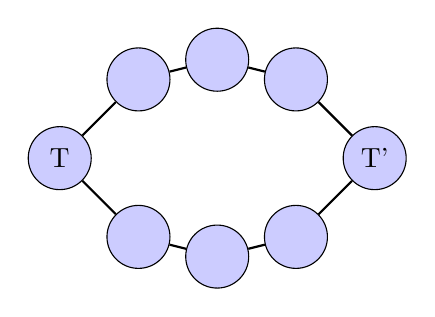
\begin{tikzpicture}[
    scale=0.5,
    node distance=1.5cm,
    every node/.style={circle, draw, fill=blue!20, minimum size=8mm}
]

% Leftmost node
\node (L) at (0,0) {T};

% Rightmost node
\node (R) at (8,0) {T'};

% Top arc nodes (concave up)
\node (T1) at (2, 2) {};
\node (T2) at (4, 2.5) {};
\node (T3) at (6, 2) {};

% Bottom arc nodes (concave down)
\node (B1) at (2, -2) {};
\node (B2) at (4, -2.5) {};
\node (B3) at (6, -2) {};

% Draw edges for top arc
\draw[thick] (L) -- (T1);
\draw[thick] (T1) -- (T2);
\draw[thick] (T2) -- (T3);
\draw[thick] (T3) -- (R);

% Draw edges for bottom arc
\draw[thick] (L) -- (B1);
\draw[thick] (B1) -- (B2);
\draw[thick] (B2) -- (B3);
\draw[thick] (B3) -- (R);

\end{tikzpicture}
    \caption{Nonunique paths in a discrete space of phylogenetic trees. Both
    central vertices are Fr\'echet means of $\{T,T'\}$.}
\label{fig:oval_graph}
\end{figure}

In such a discrete space, the Fr\'echet mean need not be unique, and distinct
means may be far apart. This is problematic if we want a single estimate
$\widehat{T}$ of the underlying species tree whose statistical properties can
be studied. Billera--Holmes--Vogtmann (BHV) space
\cite{BILLERA_2001_bhv_space} was designed in part to address this issue.

Heuristically, the BHV space $\cT_N$ of unrooted phylogenetic trees on $N$
labelled leaves is a collection of orthants $\R^{N-3}_{\geq0}$, one for each
fully resolved tree topology. Each coordinate is the length of an internal
edge. When an edge length shrinks to zero, the corresponding split disappears;
orthants containing that unresolved tree are glued along the resulting
lower-dimensional face. Each codimension-one face is incident to three maximal
orthants, corresponding to the three resolutions of a degree-four vertex. Part
of $\cT_5$ is shown in Figure~\ref{fig:bhv_5}.

\begin{figure}[t]
    \centering
    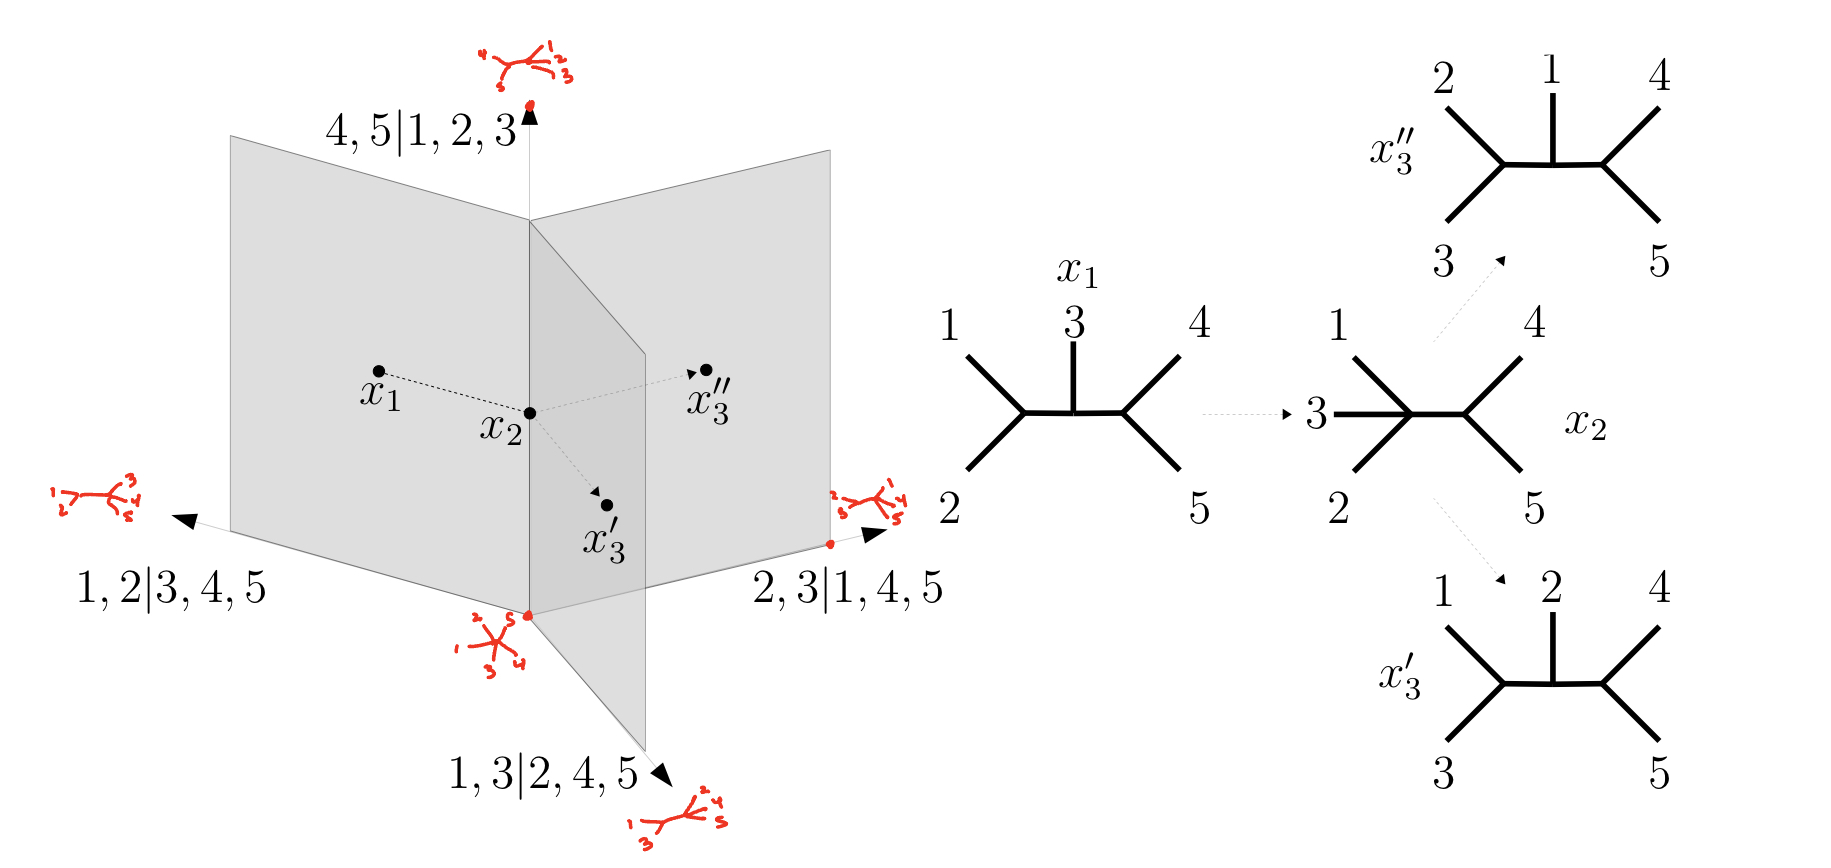
\includegraphics[width=0.8\linewidth]{images/bhv_5.jpg}
    \caption{Part of $\cT_5$, showing several orthants glued along
    lower-dimensional faces.}
    \label{fig:bhv_5}
\end{figure}

\begin{thm}
    The space $\cT_n$ is a $CAT(0)$ space. In particular, it has unique geodesics.
\end{thm}

\noindent Consequently, every finite sample has a unique empirical Fr\'echet
mean. If all branch lengths are restricted to a bounded interval, the resulting
subset of $\cT_N$ is compact, which also facilitates finite-sample concentration
around the population Fr\'echet mean.

% Brownian Motion in BHV Space
\section{Brownian Motion in BHV Space}



The Fr\'echet mean $\overline{x}$ gives a model for the "center" of our collection of trees. There are analogous ways of defining its "dispersion". For one, we could look at the sample variance:
%
\[ s^2 = \frac{1}{n-1} \sum_{i=1}^n
  d_{\mathrm{BHV}}(x_i,\overline{x})^2.\]
%

There is also a substantial literature on central limit theorems for Fr\'echet
means; see, for example, \cite{hotz2022centrallimittheoremintrinsic} and, for
stratified spaces in particular, \cite{mattingly2023centrallimittheoremsfrechet}.


A more parametric approach assumes that the trees arise from a common model and
then estimates its parameters. In Euclidean space, the classical choice would
be a Gaussian distribution. There are several inequivalent notions of what a
Gaussian should be on a singular metric space; the transition kernel of a
Brownian motion provides one natural candidate.

Nye \cite{nye2019_brownian_motion_cubical_complexes} constructs Brownian motion
on cubical complexes; BHV tree space can be treated within this framework after
subdividing its orthants into cubes. Let $I=[0,1]$. A cubical complex is a
collection of hypercubes $I^n$ glued along lower-dimensional faces, analogous
to a simplicial complex with cubes in place of simplices. It is
$n$-dimensional if it contains an $n$-cube but no higher-dimensional cube.

Inside an $n$-cube, $B_t$ should evolve as standard $n$-dimensional Brownian
motion. Upon hitting a codimension-one face $f$, it chooses uniformly among the
$n$-cubes incident to $f$ and continues there. The construction therefore has
two components:

\begin{itemize}
    \item A reflected Brownian motion in $I^n$ that dictates motion within the
    current $n$-cube.

    \item A discrete random walk on a bipartite graph $G_\cX$, with one class
    of vertices representing $n$-cubes and the other representing
    $(n-1)$-faces. An edge records incidence. This walk determines transitions
    between the $n$-cubes of $\cX$.
\end{itemize}

The main technical issue is that when we cross $f$, we will tend to recross it infinitely many times for every positive window of time afterwards before drifting away, so we have to be careful how we define our discrete random walk.  

To formalize this picture, first define reflected Brownian motion on $I^n$ by
letting its coordinates evolve independently as reflected Brownian motions on
$[0,1]$. Given a continuous path $\eta:[0,1]\to I^n$, let $\pi(\eta)$ be the
time-ordered sequence of codimension-one faces $(f_1,f_2,\ldots)$ visited by
$\eta$, with consecutive repetitions removed. We must verify that this sequence
does not make infinitely many transitions among distinct faces.

 \begin{lem}
     If $x_0\in I^n$ does not lie in a codimension-two face, then
     $\pi(\eta)$ is well-defined and finite almost surely under the law of
     $B_t$.
 \end{lem}

 \noindent Thus the discrete walk associated with a continuous Brownian path is
 almost surely well-defined and corresponds to a simple random walk on the
 incidence graph $G_\cX$.

 \begin{proof}[Proof Outline]
     Hitting a codimension-two face requires two coordinates
     $(B^i_t,B^j_t)$ to hit a specified corner simultaneously. Planar Brownian
     motion hits any fixed point with probability zero, so $\pi(\eta)$ is
     well-defined almost surely.

     To prove that $\pi(\eta)$ is almost surely finite, first restrict to paths
     that remain at least distance $\rho$ from every codimension-two face.
     Consecutive distinct faces are then separated by a positive distance, and
     uniform continuity of a Brownian path on a compact time interval rules out
     infinitely many such transitions. Finally, let $\rho\downarrow0$.
 \end{proof}

 \noindent Now we define our Brownian motion in terms of our reflected Brownian motion $W_t$ on $I^n$ as:
 %

 \begin{equation}
      \P(B_t \in A) = \sum_\omega p(\omega)\,
      \P\bigl(W_t \in \cP(A \cap \widehat{C}^{\omega})\bigr),
      \qquad p(\omega) = \prod_i \frac{1}{\deg(f_i)}
      \label{eqn:bm_on_bhv_distribution}
 \end{equation}

 %
\noindent where the sum ranges over discrete paths
$\omega=(u_0,f_1,u_1,\ldots,f_k,u_k)$ with consecutive repeated faces removed,
$\widehat{C}^{\omega}$ is the set of continuous paths inducing $\omega$, and
$\cP$ is the projection into the cubical complex. If $W_t$ has zero drift,
covariance $\sigma^2I_n$, and initial point $W_0=x_0$, then $B_t$ inherits the
source and dispersion parameters $(x_0,\sigma^2)$.

% Inference with BM
\subsection{Using Brownian Motion for Inference}

We now have a Brownian model parameterized by a source $x_0$ and dispersion
$\sigma^2$. Given sampled trees $x_1,\ldots,x_n\in\cT_N$, we would like to
estimate $(x_0,\sigma^2)$. A Bayesian approach places a prior $\pi$ on these
parameters and uses the observed trees to form their posterior distribution.

\[p(x_0,\sigma^2\mid x_1,\ldots,x_n)
  \propto \pi(x_0,\sigma^2)
  \prod_{i=1}^n p_{B_1}(x_i\mid x_0,\sigma^2).\]

\noindent Here $p_{B_1}(\,\cdot\mid x_0,\sigma^2)$ denotes the transition
density of $B_t(x_0,\sigma^2)$ at time $t=1$. This density is intractable:
Equation~\eqref{eqn:bm_on_bhv_distribution} gives a construction of the
process, but not a readily evaluable transition kernel.

Even normalizing relatively simple distributions is challenging because the
number of intersected orthants depends on the center and radius. For example,
$\cT_4$ is a tripod. The one-dimensional volume of
$B_{\mathrm{BHV}}(x_0,\epsilon)$ is
\[
  3\epsilon-\min\{d_{\mathrm{BHV}}(x_0,0),\epsilon\},
\]
as illustrated in Figure~\ref{fig:balls_in_BHV4}.


\begin{figure}[h]
    \centering
    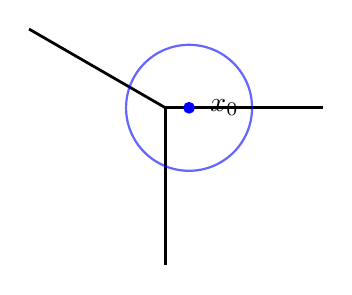
\begin{tikzpicture}[scale=2, thick]
  % Origin
  \coordinate (O) at (0,0);

  % Define directions for the three rays (orthants)
  \coordinate (A) at (1,0);
  \coordinate (B) at (150:1);
  \coordinate (C) at (270:1);

  % Draw the three orthants (black rays)
  \draw[black, line width=1pt] (O) -- (A);
  \draw[black, line width=1pt] (O) -- (B);
  \draw[black, line width=1pt] (O) -- (C);


  % Point x_0 slightly offset from origin
  \coordinate (X0) at (0.15,0);
  \filldraw[blue] (X0) circle (0.03) node[right=4pt, black] {$x_0$};

  % Draw blue "ball" around x_0 intersecting all three rays
  \draw[blue, thick, opacity=0.6] (X0) circle (0.4);

  % Optional: show distances
  %\draw[dashed, gray] (O) -- (X0) node[midway, above right] {$d_{BHV}(x_0,0)$};

\end{tikzpicture}

    \caption{An $\epsilon$-ball in $\cT_4$.}
    \label{fig:balls_in_BHV4}
\end{figure}


This problem is only exacerbated near lower-dimensional faces, where balls intersect many orthants in complicated ways. Thus we approximate $B_1$ in two steps:

\begin{enumerate}
    \item We approximate our continuous walk by a discrete walk.

    \item If the steps of our discrete walk are small enough, they typically cross at most one face (of codimension-1). In this case, the distribution of the steps is much easier to understand.
\end{enumerate}


\subsubsection{Discrete approximation using Gaussian via geodesic firing}

Suppose that $x_0$ lies in the interior of a maximal orthant. Given a
dispersion parameter $\tau^2$, define the \textit{Gaussian via geodesic firing}
distribution $GGF(x_0,\tau^2)$ as follows:

\begin{itemize}
    \item Sample a direction $v \sim N(0, \tau^2 I_{N-3})$. 
    
    \item Follow the unique geodesic starting at $x_0$ in direction $v$. 

    \item Upon reaching a codimension-one face, choose uniformly between the
    two other maximal orthants incident to that face and continue the unfolded
    geodesic in the chosen orthant.

    \item Continue until you travel total distance $|v|$.
\end{itemize}

\noindent If we iterate this process, we obtain an analog of the simple random walk with Gaussian increments. Unsurprisingly, we get the following central limit theorem.

\begin{lem}
    Let $y_0=x_0$ and sample
    $y_j\mid y_{j-1}\sim GGF(y_{j-1},\sigma^2/m)$. If
    $W(x_0,\sigma^2;m)$ denotes the distribution of $y_m$, then
    $W(x_0,\sigma^2;m)\Rightarrow B_1(x_0,\sigma^2)$ as $m\to\infty$.
\end{lem}

\noindent Hence our first approximation:

\[
  p(x_0,\sigma^2\mid\mathbf{x})
  \approx \pi(x_0,\sigma^2)
  \prod_{i=1}^n p_W(x_i\mid x_0,\sigma^2;m),
\]

\noindent up to its normalizing constant. The endpoint density $p_W$ remains
intractable because it integrates over all compatible random-walk paths. For
large $m$, however, each individual step is short and typically crosses at most
one codimension-one face, so its GGF transition density is tractable. This
motivates augmenting the model with the intermediate points of each path.

% latent paths and marginalization
\subsubsection{Latent paths and marginalization}

For observation $x_i$, write $y_{i,0}=x_0$, $y_{i,m}=x_i$, and let
$\mathbf{y}_i=(y_{i,1},\ldots,y_{i,m-1})$ be the intermediate path. The
endpoint density is the integral
\[
  p_W(x_i\mid x_0,\sigma^2;m)
  =\int \prod_{j=1}^m
  f_{GGF}\!\left(y_{i,j}\mid y_{i,j-1},\frac{\sigma^2}{m}\right)
  \,d\mathbf{y}_i.
\]
Rather than evaluate this integral directly, the paper treats the paths as
latent variables. The augmented posterior is
\[
  p(x_0,\sigma^2,\mathbf{y}_1,\ldots,\mathbf{y}_n\mid\mathbf{x})
  \propto \pi(x_0,\sigma^2)
  \prod_{i=1}^n\prod_{j=1}^m
  f_{GGF}\!\left(y_{i,j}\mid y_{i,j-1},\frac{\sigma^2}{m}\right).
\]
An MCMC algorithm can target this density without evaluating the intractable
normalizing constant. Marginalizing the sampled paths then yields posterior
samples for $(x_0,\sigma^2)$. The remaining challenge is to construct effective
proposals for paths conditioned on their two endpoints---that is, bridges.

% Sampling Bridges
\subsubsection{Sampling bridges}

The bridge proposal is inspired by the standard Brownian bridge. If
$Y_0,Y_1,\ldots,Y_m$ is a Gaussian random walk, then
%
\[
Y_j\mid\{Y_{j-1}=y_{j-1},Y_m=x^*\}
\sim N\!\left(
y_{j-1}+\frac{x^*-y_{j-1}}{m-j+1},
\frac{m-j}{m-j+1}\frac{\sigma^2}{m}I_{N-3}
\right).
\]
%
\noindent Thus the conditional mean lies a proportion $1/(m-j+1)$ of the way
from $y_{j-1}$ to $x^*$. In BHV space, the analogous basic proposal starts at
$y_0=x_0$, conditions on $y_m=x^*$, and repeats the following for
$j=1,\ldots,m-1$:

\begin{enumerate}
    \item Construct the geodesic $\Gamma_{y_{j-1},x^*}$ and let
    $\mu_j=\Gamma_{y_{j-1},x^*}(1/(m-j+1))$, where the geodesic is
    parameterized on $[0,1]$.

    \item Sample $y_j\sim GGF(\mu_j,\tau_{j,m})$, where
    $\tau_{j,m}=\frac{m-j}{m-j+1}\frac{\sigma^2}{m}$.

    \item If $\Gamma_{y_{j-1},y_j}$ is not simple---equivalently, if it meets
    a face of codimension greater than one---reject the proposal.
\end{enumerate}

\noindent This procedure is a proposal distribution, not an exact draw from
the conditional bridge law. It is embedded in a Metropolis--Hastings scheme,
whose acceptance correction targets the exact bridge distribution for the
discretized random walk.

The paper introduces several refinements to improve acceptance and guarantee
adequate proposal support, including mixture proposals and partial bridge
updates. It also treats singularities near lower-dimensional faces separately,
where the basic proposal is least reliable.

\section{Final Remarks}

The fitted source and dispersion provide analogues of the mean and variance for
a sample of trees. Once these parameters have been learned, the model can also
generate new trees for posterior prediction or downstream analysis.

Some natural questions I had after reading the article:

\begin{itemize}
    \item Under what conditions, if any, does the maximum-likelihood estimate
    of the Brownian source $x_0$ coincide with the empirical Fr\'echet mean?
    Even when they differ, fixing $x_0$ at the Fr\'echet mean could provide a
    useful approximation when estimating $\sigma^2$.

    \item Can the construction be extended to a reflected diffusion with
    nonzero drift $\mu$ and anisotropic covariance $\Sigma$, rather than
    $\mu=0$ and $\Sigma=\sigma^2I$? Such an extension would require a principled
    rule for transitions at a face. For example, a drift pointing out of the
    current cube should make continuation into a neighboring cube more likely
    than reflection back into the current one.

\end{itemize}





% Print bibliography
\newpage
\bibliographystyle{plainnat}
\bibliography{references}

\end{document}
